\documentclass[a4paper,14pt]{extarticle}

\usepackage[utf8x]{inputenc}
\usepackage[T1]{fontenc}
\usepackage[russian]{babel}
\usepackage{hyperref}
\usepackage{indentfirst}
\usepackage{here}
\usepackage{array}
\usepackage{graphicx}
\usepackage{caption}
\usepackage{subcaption}
\usepackage{chngcntr}
\usepackage{amsmath}
\usepackage{amssymb}
\usepackage[left=2cm,right=2cm,top=2cm,bottom=2cm,bindingoffset=0cm]{geometry}
\usepackage{multicol}
\usepackage{multirow}
\usepackage{titlesec}
\usepackage{listings}
\usepackage{color}
\usepackage{enumitem}
\usepackage{cmap}
\usepackage{url}

\definecolor{green}{rgb}{0,0.6,0}
\definecolor{gray}{rgb}{0.5,0.5,0.5}
\definecolor{purple}{rgb}{0.58,0,0.82}

\lstdefinelanguage{none}{}

\lstset{
	language={Java},
	backgroundcolor=\color{white},
	commentstyle=\color{green},
	keywordstyle=\color{blue},
	numberstyle=\color{gray}\scriptsize\ttfamily,
	stringstyle=\color{purple},
	basicstyle=\lst@ifdisplaystyle\footnotesize\fi\ttfamily,
	breakatwhitespace=false,
	breaklines=true,
	captionpos=b,
	keepspaces=true,
	numbers=left,
	numbersep=5pt,
	showspaces=false,
	showstringspaces=false,
	showtabs=false,
	tabsize=4,
	frame=single,
	morekeywords={},
	deletekeywords={},
	extendedchars=false,
	columns=fullflexible,
	literate=%
		{~}{{\raise.25ex\hbox{$\mathtt{\sim}$}}}{1}%
		{-}{-}{1}
}

\titleformat*{\section}{\large\bfseries} 
\titleformat*{\subsection}{\normalsize\bfseries} 
\titleformat*{\subsubsection}{\normalsize\bfseries} 
\titleformat*{\paragraph}{\normalsize\bfseries} 
\titleformat*{\subparagraph}{\normalsize\bfseries} 

\counterwithin{figure}{section}
\counterwithin{equation}{section}
\counterwithin{table}{section}
\newcommand{\sign}[1][5cm]{\makebox[#1]{\hrulefill}}
\newcommand{\code}[1]{\lstinline[language=none]|#1|}
\graphicspath{{pics/}}
\captionsetup{justification=centering,margin=1cm}
\def\arraystretch{1.3}
\setlength\parindent{5ex}
\titlelabel{\thetitle.\quad}

\setitemize{topsep=0em, itemsep=0em}
\setenumerate{topsep=0em, itemsep=0em}


\begin{document}

\begin{titlepage}
\begin{center}
	Санкт-Петербургский Политехнический Университет Петра Великого\\[0.3cm]
	Институт компьютерных наук и технологий \\[0.3cm]
	Кафедра компьютерных систем и программных технологий\\[4cm]
	
	\textbf{ОТЧЕТ}\\ 
	\textbf{по лабораторной работе}\\[0.5cm]
	\textbf{<<Создание многопроцессного приложения средствами MPI>>}\\[0.1cm]
	Параллельные вычисления\\[3.0cm]
\end{center}

\begin{flushright}
	\begin{minipage}{0.5\textwidth}
		\textbf{Работу выполнил студент}\\[3mm]
		гр. 3540901/91502 \hfill \sign[1.1cm] \hfill Дьячков В.В.\\[5mm]
		\textbf{Работу принял преподаватель}\\[5mm]
		\sign[2cm] \hfill к.т.н., доц. Стручков И.В. \\[5mm]
	\end{minipage}
\end{flushright}

\vfill

\begin{center}
	Санкт-Петербург\\[0.3cm]
	\the\year
\end{center}
\end{titlepage}

\addtocounter{page}{1}


\tableofcontents
\newpage

\section{Индивидуальное задание}

\paragraph{Варинат 10.} Определить частоту встречи слов в тексте на русском языке при помощи многопроцессного MPI-приложения. 

\section{Используемое окружение}

\begin{itemize}
	\item ОС: macOS Catalina
	\item Версия ОС: 10.15.4
	\item Процессор: Intel Core i9 @ 2.3GHz × 8
	\item ОЗУ: 16 ГБ
	\item OpenJDK 14
	\item OpenMPI 4.0.3 
\end{itemize}

\section{Алгоритм решения}

Разработку было решено вести на языке Java, с использованием bindings, предоставляемых библиотекой OpenMPI.

Общий интерфейс для поиска частоты вхождения N-грамм можно описать следующим образом:

\begin{lstlisting}
public interface NGramFinder {
	@NotNull
	Map<String, Integer> findNGrams(String[] files) throws Exception;
}
\end{lstlisting}

На вход программе подается набор текстовых файлов, на основе которых и нужно вычислить вероятность появления N-грамм. При этом последовательный алгоритм производит обработку каждого файла последовательно, в то вермя как параллельный алгоритм с использованием OpenMPI разбивает файлы поровну между процессами, уменьшая при этом объем работы одного процесса.

Выходным значением функции является отображение N-граммы на число ее вхождений в переданные текстовые файлы. Для удобства, общее число рассмотренных токенов сохраняется в том же отображении, и используется для вычисления вероятности появления N-граммы $p_{gram}$:
$$
p_{gram} = \dfrac{N_{gram}}{N_{tokens}}
$$

Рассмотрим архитектуру разработанного Java-прилжения. 

\begin{figure}[H]
	\centering
	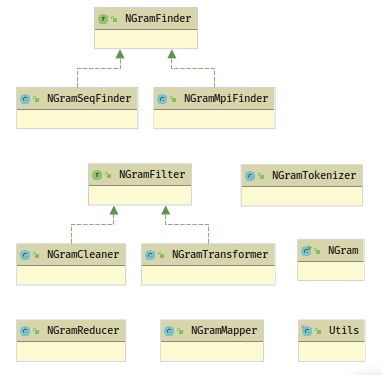
\includegraphics[width=0.6\linewidth]{classes}
	\caption{Разработанные классы}
\end{figure}

\begin{itemize}
	\item \code{NGram.java} -- класс, содержащий метод \code{main}, который инстаниирует последовательную или паралельную версию определения частот N-грамм.
	\item \code{NGramFinder.java} -- интерфейс, описывающий решаему задчу:
		\begin{itemize}
			\item \code{NGramSeqFinder.java} -- класс, решающий задачу последовательно;
			\item \code{NGramMpiFinder.java} -- класс, использующий интерфейс MPI для обмена инфрмации с другими процессами.
		\end{itemize}
	\item \code{NGramFilter.java} -- интерфейс, описывающий этап фильтрации входного текста:
		\begin{itemize}
			\item \code{NGramCleaner.java} -- класс, удаляющий из входного потока некириллические символы (латиница, пунктуация и т.д.)
			\item \code{NGramTransformer.java} -- класс, применяющий трансформацию к тексу (смена регистра, "схлопывание" пробелов и т.д.)
		\end{itemize}
	\item \code{NGramTokenizer.java} -- класс, разбивающий входной текст на N-граммы.
	\item \code{Utils.java} -- класс, содержащий служебные функции.
\end{itemize}

\noindent Наиболее частотными 3-граммами в рассматриваемых текстах оказались:
\begin{itemize}
	\item что: 0.42\%;
	\item его: 0.37\%;
	\item ост: 0.33\%;
	\item ого: 0.32\%;
	\item про: 0.30\%.
\end{itemize} 

\section{Эксперименты}

В качестве исходных текстов использовались 16 произведений классической русской литературы, такие как ''Война и мир'', ''Анна Каренина'' и др. Для эмуляции большого количества данных, дополнительно были проведены эксперименты, в которых один и тот же файл передавался в качестве входного 10 и 20 раз соответственно.

Число рассматриваемых процессов -- 1 (последовательное выполнение) и от 2 до 16 с шагом в 2 (параллельное выполнение). Для каждого числа процессов измерение времени выполнения было произведено 10 раз, чтобы уменьшить случайность в получаемых данных. 

Для каждого измеренного времени было посчитано ускорение в сравнении с последовательной версией выполнения алгоритма.

\begin{figure}[H]
	\centering
	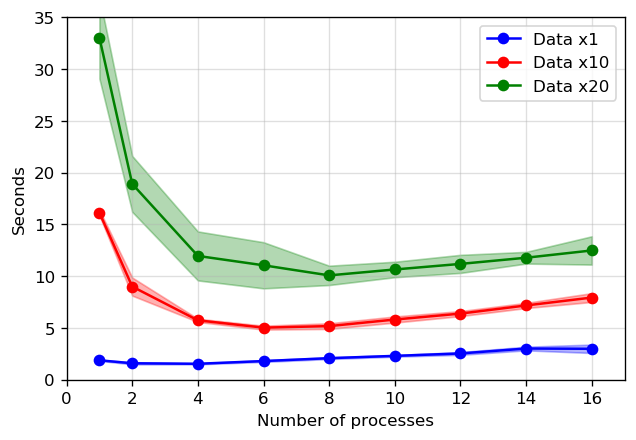
\includegraphics[width=0.85\linewidth]{all}
	\caption{Время поиска частот N-грамм в зависимости от числа процессов и объема данных}
\end{figure}

\begin{figure}[H]
	\centering
	\begin{subfigure}{0.5\linewidth}
		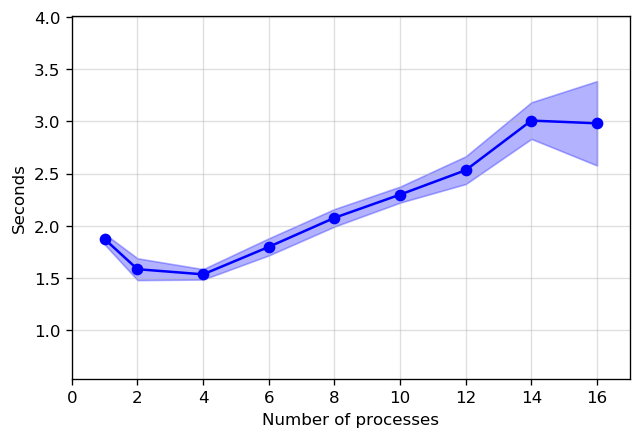
\includegraphics[width=\linewidth]{1}
		\caption{\code{Data x1}}
	\end{subfigure}
	\begin{subfigure}{0.49\linewidth}
		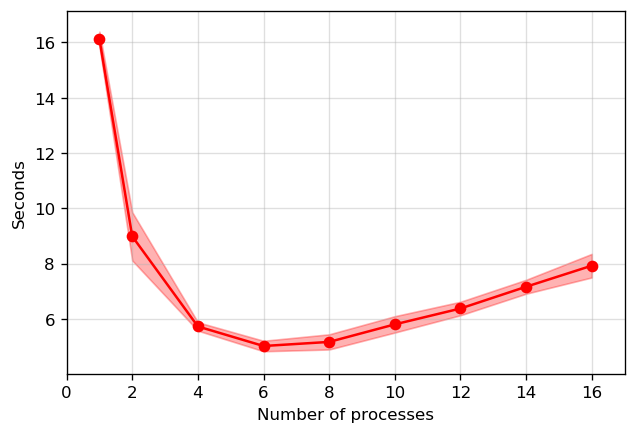
\includegraphics[width=\linewidth]{10}
		\caption{\code{Data x10}}
	\end{subfigure}
	\begin{subfigure}{0.49\linewidth}
		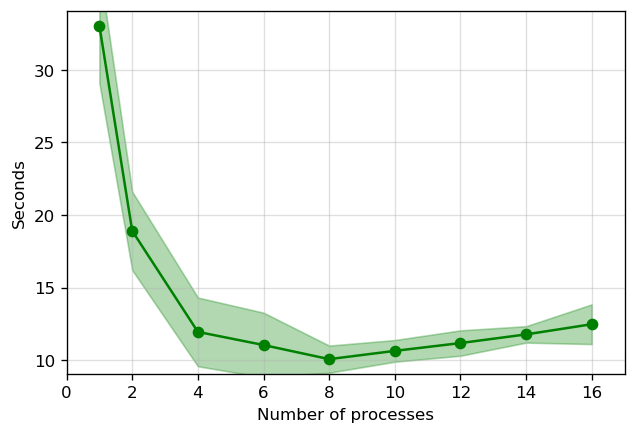
\includegraphics[width=\linewidth]{20}
		\caption{\code{Data x20}}
	\end{subfigure}
\end{figure}

\begin{figure}[H]
	\centering
	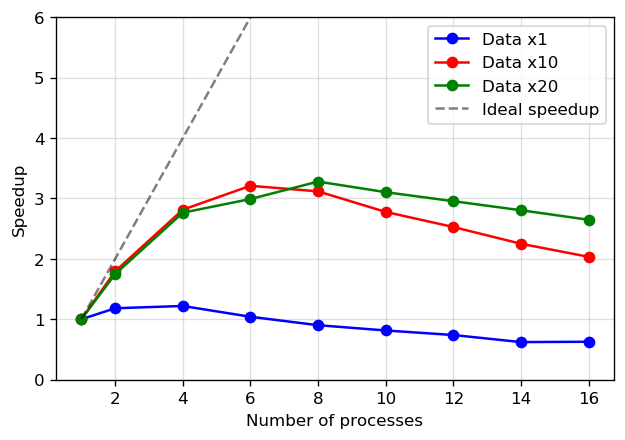
\includegraphics[width=0.85\linewidth]{speedup}
	\caption{Ускорение в зависимости от числа процессов и объема данных}
\end{figure}

Из графиков видно, что при небольшом объеме данных (\code{Data x2}), использование OpenMPI почти не ускоряе выполнение программы, а при числе процессов больше 6 и вовсе замедляет. Время выполнения при этом составляетот 1.5 до 3 секунд.

При среднем (\code{Data x10}) и большом (\code{Data x20}) объеме данных, распараллеливание позволяет значительно ускорить программу (примерно в 3.2 раза), снизив время выполнения с 16 и 32 секунд до 5 и 10 секунд соответстветнно. Оптимальным числом процессов при этом является 6 и 8 соответственно.

Большее ускорение, возможно, не может быть достигнуто ввиду активной работе с дисковой подсистемой в процессе обработки исходных текстов. Данная проблема могла бы быть устранена в случае использования распределенной файловой системы (например, HDFS), и запуска программы на разных узлах MPI-кластера.

\section{Выводы}

В рамках данной лабораторной работы:

\begin{itemize}
	\item разработано Java-приложение, вычисляющее вероятность появления N-грамм в тексте на русском языке;
	\item для распараллеливания исходной задачи использована библиотека OpenMPI;
	\item достигнуто ускорение в 3.2 раза параллельной версии в сравении с последовательной.
\end{itemize}

\end{document}